\documentclass{article}
\usepackage{neurips_2026}
\usepackage[utf8]{inputenc}
\usepackage[T1]{fontenc}
\usepackage{microtype}
\usepackage{booktabs}
\usepackage{amsmath,amssymb,mathtools}
\usepackage{graphicx}
\usepackage{multirow}
\usepackage{tabularx}
\usepackage{array}
\usepackage{enumitem}
\usepackage{url}
\usepackage{hyperref}
\usepackage{tikz}
\setlength{\textfloatsep}{7pt plus 2pt minus 2pt}
\setlength{\floatsep}{6pt plus 2pt minus 2pt}
\setlength{\intextsep}{6pt plus 2pt minus 2pt}
\setlength{\abovecaptionskip}{4pt}
\setlength{\belowcaptionskip}{0pt}
\usetikzlibrary{arrows.meta,positioning,fit}
\hypersetup{colorlinks=true,citecolor=blue,linkcolor=blue,urlcolor=blue}
\setlist[itemize]{leftmargin=1.25em,itemsep=1pt,topsep=2pt}
\setlist[enumerate]{leftmargin=1.35em,itemsep=1pt,topsep=2pt}
\newcolumntype{Y}{>{\centering\arraybackslash}X}
\newcommand{\OL}{\mathrm{OL}}
\newcommand{\CL}{\mathrm{CL}}
\newcommand{\obs}[1]{\textsc{#1}}
\newcommand{\figdir}{figures}

\title{Beyond Replay RMSE: Auditing Offline Selection of Learned State Observers for Closed-Loop Robot Control}
\author{Anonymous Authors}

\begin{document}
\maketitle

\begin{abstract}
Learned state observers are usually trained and selected using estimation error on fixed trajectories, even though deployment places them inside a feedback loop. We study the resulting proxy mismatch for differential-drive tracking with biased odometry and intermittent range--bearing sensing. Six deployment candidates---dead reckoning, an extended Kalman filter (EKF), and GRU or selective state-space residual observers anchored to either model---are evaluated through paired common-input replay and closed-loop rollouts over 24 degradation conditions. Replay position RMSE preserves broad ordering (Spearman $\rho=0.923$) but selects a suboptimal closed-loop observer in $5/24$ conditions. We formulate observer selection through top-1 agreement and closed-loop regret, then test three task-aware offline alternatives: exact controller-command disagreement, a local controller-sensitivity error, and counterfactual error replay. The sensitivity score reduces observed failures to $3/24$, but its bootstrap interval overlaps no improvement and its worst regret is larger; the other proxies perform worse. Matched EKF-anchor ablations show that selectivity is regime-dependent rather than universally stabilizing, while three training initializations reveal substantial stress-regime variability. A second controller changes the oracle observer in $8/24$ conditions. Finally, 600 seconds of UTIAS MRCLAM physical logs expose poor zero-shot map transfer from the ordered landmark-slot representation. We release a reproducible evaluation protocol that treats observer deployment as a decision problem: report replay and closed-loop metrics, top-1 agreement, selection regret, matched ablations, training-seed uncertainty, controller dependence, and physical-log stress tests.
\end{abstract}

\section{Introduction}
State estimation is usually evaluated as an isolated prediction problem. A filter receives controls and measurements, produces a pose, and is ranked by position or heading root-mean-square error (RMSE) against ground truth. In an autonomous system, however, the estimate is consumed by a controller. The resulting command changes the future state, which changes the next measurement and therefore the future estimator input. This feedback creates two gaps between replay accuracy and deployment utility: errors are directionally weighted by the controller, and the estimator induces its own closed-loop data distribution.

This distinction is especially important for learned observers. Recurrent filters can exploit temporal patterns and model mismatch, but they can also learn corrections that are benign on expert-generated logs and destabilizing when their own errors alter the trajectory. Closely related objective mismatch has been documented for learned dynamics models in model-based reinforcement learning~\citep{lambert2020objective}; here we isolate it at the observer layer. The question is not whether replay RMSE is correlated with control---it generally is---but whether it reliably supports the actual model-selection decision.

We study a controlled yet nontrivial setting: a differential-drive robot follows a figure-eight using biased, noisy wheel odometry and intermittent range--bearing measurements to a known landmark map. The candidate set spans classical and hybrid estimators: dead reckoning, an EKF~\citep{thrun2005probabilistic}, and recurrent residual observers with GRU or selective diagonal state-space cores inspired by S4 and Mamba~\citep{gu2022s4,gu2024mamba}. Residuals are anchored either to dead reckoning or to the EKF, allowing us to separate recurrent architecture from analytic prior strength.

Our contribution is an evaluation framework rather than a claim that one recurrent cell dominates. Specifically, we provide:
\begin{itemize}
\item a paired replay/closed-loop benchmark with six observers, four physical degradation axes, 24 conditions, and ten evaluation seeds;
\item a decision-theoretic analysis using top-1 agreement, absolute regret, and relative regret, rather than correlation alone;
\item three controller-aware offline proxy baselines and an empirical demonstration that task awareness does not automatically yield deployment-valid selection;
\item matched same-anchor ablations, a three-training-seed robustness study, and a matched pure-pursuit/Kanayama controller sensitivity analysis;
\item physical-log localization and deliberately difficult zero-shot transfer on UTIAS MRCLAM~\citep{leung2011utias}, plus a real-noise-calibrated closed-loop replay.
\end{itemize}
The central finding is nuanced: replay position RMSE is an informative coarse proxy, but it does not eliminate the need for a small, stratified closed-loop evaluation.

\section{Related work}
\paragraph{Classical and learned state estimation.}
The EKF remains a standard nonlinear localization baseline~\citep{thrun2005probabilistic}. Learned estimators range from discriminative recurrent filters~\citep{ha2016backprop} and variational state-space models~\citep{karl2017dvbf,rubanova2019latentode} to architectures that preserve algorithmic structure, including recurrent Kalman networks~\citep{becker2019rkn}, differentiable particle filters~\citep{jonschkowski2018dpf}, and KalmanNet~\citep{revach2022kalmannet}. Our residual observers follow this hybrid philosophy but focus on how candidates are selected for feedback deployment.

\paragraph{State-space sequence models.}
Structured state-space models provide efficient long-context recurrences~\citep{gu2022s4}; selective SSMs make transition and input parameters depend on the current token~\citep{gu2024mamba}. Intermittent sensing appears naturally suited to selectivity because the observer should adapt retention and correction when measurements vanish or reappear. We test that intuition with a compact diagonal selective cell and, importantly, with matched non-selective and mask-free controls.

\paragraph{Task-aware evaluation and proxy mismatch.}
Pure pursuit~\citep{coulter1992pure} and Kanayama tracking~\citep{kanayama1990stable} map pose errors into actions differently, so an estimator's utility can be controller-specific. Proxy mismatch in model-based RL~\citep{lambert2020objective} motivates our emphasis on selection regret. Unlike work proposing a single task-aware loss, we compare several offline surrogates and report their failure modes.

\section{Closed-loop observer selection}
\subsection{Robot, sensing, and feedback}
The robot state is $s_t=(x_t,y_t,\theta_t)$ and the commanded input is $u_t=(v_t,\omega_t)$. With step size $\Delta t=0.1$ s,
\begin{equation}
\begin{aligned}
x_{t+1}&=x_t+\Delta t\,v_t\cos\theta_t,\\
y_{t+1}&=y_t+\Delta t\,v_t\sin\theta_t,\\
\theta_{t+1}&=\mathrm{wrap}(\theta_t+\Delta t\,\omega_t).
\end{aligned}
\end{equation}
Odometry contains multiplicative linear-velocity slip, additive angular-rate bias, and Gaussian noise:
$\tilde v_t=\kappa v_t+\epsilon^v_t$ and $\tilde\omega_t=\omega_t+b_g+\epsilon^\omega_t$.
Visible landmark $j$ yields noisy range and bearing
$z_{t,j}=(\|p_j-p_t\|+\epsilon^r,\,\mathrm{atan2}(p_j-p_t)-\theta_t+\epsilon^b)$.
A periodic schedule removes all exteroceptive measurements during blackouts; a mask indicates which landmark slots are present.

The controller is $u_t=\pi(\hat s_t,t)$, where $\hat s_t$ is the observer output. Thus the closed-loop state distribution depends on the candidate observer. Figure~\ref{fig:protocol} contrasts common-input replay with the deployment loop.

\begin{figure}[t]
\centering
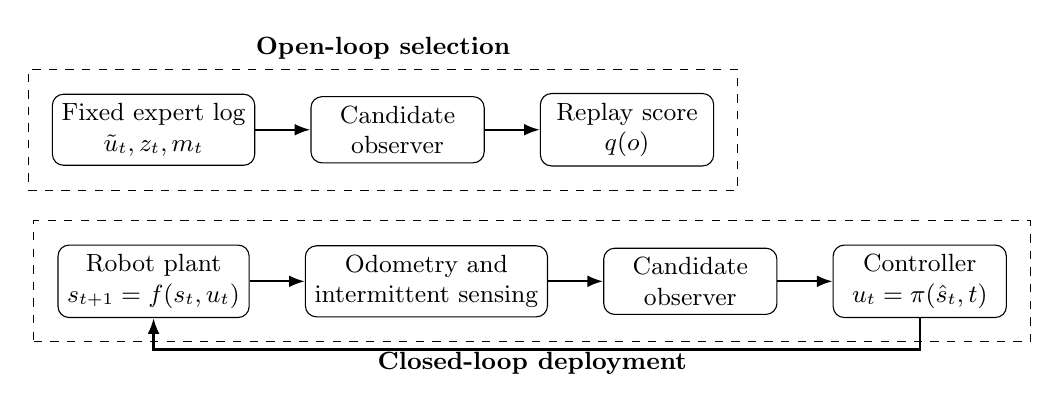
\begin{tikzpicture}[node distance=5.5mm and 7mm, every node/.style={font=\small}, box/.style={draw,rounded corners,align=center,minimum height=8mm,minimum width=22mm}, arr/.style={-{Latex[length=2mm]},thick}]
\node[box] (log) {Fixed expert log\\$\tilde u_t,z_t,m_t$};
\node[box,right=of log] (obs1) {Candidate\\observer};
\node[box,right=of obs1] (rmse) {Replay score\\$q(o)$};
\draw[arr] (log)--(obs1); \draw[arr] (obs1)--(rmse);
\node[box,below=10mm of log] (plant) {Robot plant\\$s_{t+1}=f(s_t,u_t)$};
\node[box,right=of plant] (sense) {Odometry and\\intermittent sensing};
\node[box,right=of sense] (obs2) {Candidate\\observer};
\node[box,right=of obs2] (ctrl) {Controller\\$u_t=\pi(\hat s_t,t)$};
\draw[arr] (plant)--(sense); \draw[arr] (sense)--(obs2); \draw[arr] (obs2)--(ctrl);
\draw[arr] (ctrl.south) |- ++(0,-4mm) -| (plant.south);
\node[fit=(log)(rmse),draw,dashed,inner sep=3mm,label=above:{\bf Open-loop selection}] {};
\node[fit=(plant)(ctrl),draw,dashed,inner sep=3mm,label=below:{\bf Closed-loop deployment}] {};
\end{tikzpicture}
\caption{Replay holds inputs fixed, while closed-loop evaluation lets observer errors alter actions, states, and future measurements.}
\label{fig:protocol}
\end{figure}

\subsection{Observer selection as a decision problem}
Let $\mathcal O$ be the candidate set, $c$ an operating condition, $q_c(o)$ an offline score, and $J_c(o)$ the closed-loop cross-track RMSE. The proxy-selected and oracle observers are
\begin{equation}
 o^*_{q,c}=\arg\min_{o\in\mathcal O} q_c(o),\qquad
 o^*_{\CL,c}=\arg\min_{o\in\mathcal O} J_c(o).
\end{equation}
We report top-1 failure $\mathbb{1}[o^*_{q,c}\neq o^*_{\CL,c}]$, absolute regret
$\mathcal R_{q,c}=J_c(o^*_{q,c})-J_c(o^*_{\CL,c})$, and relative regret $\mathcal R_{q,c}/J_c(o^*_{\CL,c})$. This explicitly evaluates the deployment decision; a high global correlation can coexist with repeated top-1 errors.

\section{Observer models and offline proxies}
\subsection{Analytic and residual observers}
Dead reckoning integrates $\tilde u_t$. The EKF uses the same unicycle motion model and masked range--bearing updates. A learned observer first advances an analytic anchor $\bar s_t$ and then predicts a residual:
\begin{equation}
 h_t=\mathcal G_\psi(h_{t-1},\phi_t),\qquad
 \hat s_t=\bar s_t\oplus W_o h_t.
\end{equation}
The feature $\phi_t$ contains odometry increments; eight ordered tuples $(r_j,\sin b_j,\cos b_j,m_j)$; a global measurement-presence bit; anchor position and sinusoidal heading; and, for EKF-anchored models, the covariance diagonal. The near-zero readout initialization makes the initial model approximately equal to its anchor.

For the selective diagonal SSM, with $A=-\mathrm{softplus}(a)$,
\begin{equation}
\begin{aligned}
\Delta_t&=\mathrm{softplus}(W_\Delta\phi_t+b_\Delta),\quad
B_t=W_B\phi_t+b_B,\quad C_t=W_C\phi_t+b_C,\\
\bar A_t&=\exp(\Delta_t\odot A),\\
h_t&=\bar A_t\odot h_{t-1}+(\Delta_t\odot B_t)\odot(W_{\mathrm{in}}\phi_t),\\
r_t&=W_o(C_t\odot h_t)+b_o.
\end{aligned}
\end{equation}
The non-selective ablation replaces $\Delta_t,B_t,C_t$ by learned constants. This is a compact selective recurrence, not a full Mamba block.

\begin{table}[t]
\centering
\caption{Principal observer set. All learned models use hidden size 32 and the same residual loss.}
\label{tab:zoo}
\small
\begin{tabular}{lcccc}
\toprule
Observer & Anchor & Recurrent core & Covariance input & Parameters\\
\midrule
\obs{DR} & Dead reckoning & -- & -- & --\\
\obs{EKF} & EKF & -- & internal & --\\
\obs{GRU-DR} & Dead reckoning & GRU & no & 7,011\\
\obs{SSM-DR} & Dead reckoning & selective SSM & no & 5,219\\
\obs{GRU-EKF} & EKF & GRU & yes & 7,299\\
\obs{SSM-EKF} & EKF & selective SSM & yes & 5,603\\
\bottomrule
\end{tabular}
\end{table}

\subsection{Controller-aware offline proxies}
Position and heading RMSE ignore the downstream map from pose to action. We additionally test three log-only proxies. Let $e_t=\hat s_t\ominus s_t$, $D$ normalize action units, and $J_\pi(s_t,t)$ be a finite-difference controller Jacobian.
\begin{align}
q_{\mathrm{cmd}}(o)&=\left[\frac1T\sum_t\|D^{-1}(\pi(\hat s_t,t)-\pi(s_t,t))\|_2^2\right]^{1/2},\\
q_{\mathrm{LCSE}}(o)&=\left[\frac1T\sum_t\|D^{-1}J_\pi(s_t,t)e_t\|_2^2\right]^{1/2}.
\end{align}
Counterfactual error replay injects the logged error sequence $e_t$ into a shadow plant and evaluates the tracking error produced by the controller. It captures temporal accumulation but still freezes the observer error trace, so it does not reproduce full feedback adaptation.

\section{Experimental design}
\paragraph{Training.}
Each recurrent observer is trained on 200 expert-controlled trajectories of 200 steps, with a separate validation set. Every trajectory randomizes path amplitude, slip, gyro bias, range/bearing noise, blackout length and period, and active landmark count. We use hidden size 32, Adam, gradient clipping at 5, batch size 24, 32 epochs, and retain the best validation checkpoint. The loss is squared position error plus $0.5(1-\cos\Delta\theta)$.

\paragraph{Synthetic evaluation.}
The reference contains 220 steps. At each of 24 conditions, the six observers are evaluated over ten fresh seeds in both common-input replay and closed loop. One degradation variable is swept while all others remain nominal. Table~\ref{tab:protocol} lists the full design. Closed-loop metrics include cross-track and pose RMSE, maximum cross-track error, angular-control effort, post-blackout recovery time, and divergence fraction.

\begin{table}[t]
\centering
\caption{Evaluation protocol. Range-noise sweeps use bearing noise $\sigma_b=0.5\sigma_r$.}
\label{tab:protocol}
\small
\begin{tabularx}{\linewidth}{lX}
\toprule
Component & Values\\
\midrule
Nominal sensing & slip $0.92$; gyro bias $0.06$ rad/s; $\sigma_r=0.12$ m; $\sigma_b=0.06$ rad; blackout 14/45 steps; 6 landmarks\\
Blackout sweep & 4, 10, 16, 22, 28, 34 steps\\
Range-noise sweep & $\sigma_r\in\{0.05,0.12,0.20,0.30,0.40,0.50\}$ m\\
Landmark sweep & 2, 3, 4, 5, 6, 8 active landmarks\\
Gyro-bias sweep & 0, 0.05, 0.10, 0.15, 0.20, 0.25 rad/s\\
Primary controller & pure pursuit, $v_{\rm cmd}=1.0$ m/s, lookahead $0.8$ m\\
Secondary controller & Kanayama tracking, matched plant, limits, checkpoints, and five seeds\\
Uncertainty & 95\% CI across evaluation seeds; condition bootstrap for selection; three SSM-EKF training seeds\\
\bottomrule
\end{tabularx}
\end{table}

\paragraph{Physical logs.}
UTIAS MRCLAM contains synchronized odometry, range--bearing observations, known landmark positions, and Vicon ground truth~\citep{leung2011utias}. We align a 600 s segment of Dataset 1 Robot 1 to 6,000 samples with 1,878 observations. We evaluate dead reckoning, a $3\times3$ EKF covariance grid, and zero-shot learned models on an eight-landmark subset. A separate synthetic replay resamples empirical sensor residuals and the physical observation-count sequence; it is not presented as hardware closed-loop control.

\paragraph{Statistics.}
We compute global Spearman/Pearson associations over $24\times6$ condition-observer pairs, per-condition rank agreement, top-1 failures, and selection regret. Confidence intervals for proxy selection resample the 24 conditions. Matched ablations use paired evaluation seeds. The controller comparison bootstraps the five matched seeds and is reported as a sensitivity analysis.

\section{Results}
\subsection{Nominal performance and degradation regimes}
Table~\ref{tab:nominal} shows the nominal operating point. EKF-anchored learned observers are the only learned models that remain consistently stable. GRU-EKF attains the best replay and closed-loop performance, reducing cross-track RMSE from $0.212$ m for EKF to $0.163$ m. In contrast, GRU-DR and SSM-DR improve replay RMSE by factors of 4--5 relative to dead reckoning while retaining much larger closed-loop error and divergence. This is an immediate example of an improvement that does not survive feedback.

\begin{table*}[t]
\centering
\caption{Nominal evaluation over ten seeds, mean $\pm$ 95\% CI half-width. Lower is better. ``Div.'' is the fraction of steps outside the 1 m tracking tube.}
\label{tab:nominal}
\small
\resizebox{\textwidth}{!}{%
\begin{tabular}{lccccccc}
\toprule
Observer & Replay pos. & Replay head. & CL cross-track & CL pose & Max cross-track & Effort $\overline{\omega^2}$ & Div.\\
 & (m) & (rad) & (m) & (m) & (m) &  & \\
\midrule
\obs{DR} & $1.503\pm0.200$ & $0.832\pm0.022$ & $1.045\pm0.025$ & $1.834\pm0.040$ & $2.557\pm0.062$ & $0.449\pm0.063$ & $0.260$\\
\obs{EKF} & $0.140\pm0.009$ & $0.092\pm0.006$ & $0.212\pm0.018$ & $0.146\pm0.006$ & $0.628\pm0.153$ & $0.681\pm0.128$ & $0.004$\\
\obs{GRU-DR} & $0.281\pm0.031$ & $0.359\pm0.087$ & $0.694\pm0.345$ & $1.033\pm0.371$ & $1.718\pm0.781$ & $0.914\pm0.129$ & $0.140$\\
\obs{SSM-DR} & $0.325\pm0.039$ & $0.276\pm0.038$ & $0.909\pm0.498$ & $1.399\pm0.809$ & $2.016\pm0.947$ & $1.123\pm0.120$ & $0.195$\\
\obs{GRU-EKF} & $\mathbf{0.094\pm0.012}$ & $0.093\pm0.015$ & $\mathbf{0.163\pm0.022}$ & $\mathbf{0.109\pm0.013}$ & $\mathbf{0.573\pm0.085}$ & $0.949\pm0.128$ & $0.000$\\
\obs{SSM-EKF} & $0.121\pm0.018$ & $\mathbf{0.090\pm0.013}$ & $0.199\pm0.033$ & $0.191\pm0.043$ & $0.684\pm0.076$ & $1.052\pm0.136$ & $0.000$\\
\bottomrule
\end{tabular}}
\end{table*}

Figure~\ref{fig:sweeps} reveals that the best closed-loop observer is regime-dependent. GRU-EKF dominates moderate blackouts and most noise/bias levels. Plain EKF becomes preferable at the two longest blackouts, where learned correction has little information to exploit. SSM-EKF is strongest with two active landmarks and is competitive under high range noise and bias. DR-anchored recurrent models degrade sharply as blackout duration and bias grow.

\begin{figure*}[t]
\centering
\begin{minipage}[t]{0.49\textwidth}\centering

\includegraphics[width=\linewidth]{\figdir/fig_sweep_blackout_compact.png}
\end{minipage}\hfill
\begin{minipage}[t]{0.49\textwidth}\centering

\includegraphics[width=\linewidth]{\figdir/fig_sweep_range_noise_compact.png}
\end{minipage}
\vspace{1mm}
\begin{minipage}[t]{0.49\textwidth}\centering

\includegraphics[width=\linewidth]{\figdir/fig_sweep_landmarks_compact.png}
\end{minipage}\hfill
\begin{minipage}[t]{0.49\textwidth}\centering

\includegraphics[width=\linewidth]{\figdir/fig_sweep_gyro_bias_compact.png}
\end{minipage}
\caption{Corrected six-observer closed-loop sweeps, mean $\pm$ 95\% CI over ten evaluation seeds. No single learned architecture is uniformly best.}
\label{fig:sweeps}
\end{figure*}

\subsection{Replay accuracy is correlated with control, but not decision-complete}
Across all 144 condition-observer pairs, replay position RMSE has Spearman $\rho=0.923$ and Pearson $r=0.477$ with closed-loop cross-track error (Figure~\ref{fig:scatter}). The high rank correlation means replay evaluation is useful for coarse screening. The weaker magnitude correlation and top-1 failures mean it is insufficient for final deployment selection.

\begin{figure*}[t]
\centering
\begin{minipage}[t]{0.56\textwidth}\centering

\includegraphics[width=\linewidth]{\figdir/fig_proxy_scatter_compact.png}
\end{minipage}\hfill
\begin{minipage}[t]{0.42\textwidth}\centering

\includegraphics[width=\linewidth]{\figdir/fig_proxy_failures_compact.png}
\end{minipage}
\caption{Left: replay position RMSE versus closed-loop tracking over all 144 condition-observer pairs. Right: top-1 deployment failures for five offline proxies.}
\label{fig:scatter}
\end{figure*}

Replay position RMSE selects a different observer than the closed-loop oracle in $5/24$ conditions: the two longest blackouts, the two highest range-noise levels, and the eight-landmark endpoint. Mean regret is 0.0051 m and maximum regret is 0.0347 m (12.7\% relative). These numbers are modest in this low-speed simulation, but the pattern is systematic: replay favors SSM-EKF when EKF or GRU-EKF has lower tracking error.

\begin{table}[t]
\centering
\caption{Offline proxy quality against closed-loop cross-track RMSE. Failure and regret intervals bootstrap the 24 conditions.}
\label{tab:proxies}
\small
\begin{tabular}{lccccc}
\toprule
Proxy & $\rho$ & Failures & Failure CI & Mean regret & Max\\
\midrule
Position RMSE & .923 & 5/24 & [.083,.375] & .0051 & .0347\\
Heading RMSE & .881 & 19/24 & [.625,.958] & .0237 & .0474\\
Command disagreement & .876 & 13/24 & [.333,.750] & .0188 & .1208\\
LCSE & .903 & 3/24 & [.000,.250] & .0051 & .0940\\
Counterfactual replay & .842 & 14/24 & [.375,.792] & .0159 & .0474\\
\bottomrule
\end{tabular}
\end{table}

LCSE reduces the observed failure count from five to three by accounting for controller anisotropy, but the paired bootstrap interval for failure-fraction reduction is $[-0.125,0.292]$. Its two-landmark failure incurs 0.094 m regret, larger than the worst replay-RMSE failure. Exact command disagreement is worse because action similarity at a fixed state does not capture future state and sensing changes; counterfactual replay likewise freezes the observer error trace. Controller awareness therefore shifts rather than eliminates failure regimes.

\paragraph{Compound stress.}
When all axes are simultaneously hard, GRU-EKF is best in replay and closed loop (Table~\ref{tab:compound}). The sharper counterexample is within SSM-EKF: relative to EKF it reduces replay position RMSE by 43\% ($0.829\rightarrow0.472$ m) yet increases closed-loop cross-track RMSE by 10\% ($1.324\rightarrow1.459$ m). Therefore, a large real replay improvement for a particular observer need not transfer to control.

\begin{table}[t]
\centering
\caption{Compound-stress evaluation, mean $\pm$ 95\% CI.}
\label{tab:compound}
\small
\begin{tabular}{lccc}
\toprule
Observer & Replay pose (m) & CL pose (m) & CL cross-track (m)\\
\midrule
\obs{DR} & $3.289\pm0.382$ & $4.818\pm0.030$ & $2.528\pm0.014$\\
\obs{EKF} & $0.829\pm0.066$ & $1.467\pm0.358$ & $1.324\pm0.094$\\
\obs{GRU-EKF} & $\mathbf{0.447\pm0.049}$ & $\mathbf{1.222\pm0.422}$ & $\mathbf{1.052\pm0.326}$\\
\obs{SSM-EKF} & $0.472\pm0.044$ & $1.496\pm0.350$ & $1.459\pm0.156$\\
\obs{SSM-DR} & $0.798\pm0.099$ & $5.734\pm1.419$ & $4.228\pm1.360$\\
\bottomrule
\end{tabular}
\end{table}

\subsection{Matched ablations: the anchor is more consistent than selectivity}
A valid selectivity ablation must keep the analytic anchor, inputs, hidden size, and training protocol fixed. Table~\ref{tab:ablation} compares three EKF-anchored SSMs. Nominal performance is nearly identical. Selectivity helps under high gyro bias but hurts under long blackouts and sparse sensing. Removing the global mask bit has little effect because each landmark tuple already contains a local mask. The robust qualitative factor is the EKF anchor: DR-anchored learned models are much less stable despite competitive replay error.

\begin{table}[t]
\centering
\caption{Matched EKF-anchor ablation: closed-loop cross-track RMSE (m). Bold is best per condition.}
\label{tab:ablation}
\small
\begin{tabular}{lccc}
\toprule
Condition & Selective+mask & Non-selective & No global mask\\
\midrule
Nominal & 0.199 & 0.203 & \textbf{0.195}\\
Long blackout & 0.336 & \textbf{0.235} & 0.308\\
High range noise & 0.307 & 0.322 & \textbf{0.294}\\
Two landmarks & 0.289 & \textbf{0.235} & 0.274\\
High gyro bias & 0.314 & 0.393 & \textbf{0.312}\\
\bottomrule
\end{tabular}
\end{table}



\subsection{Training uncertainty and controller dependence}
The three SSM-EKF initializations have nominal means from 0.189 to 0.199 m, but long-blackout means from 0.231 to 0.336 m and high-noise means from 0.249 to 0.307 m. Evaluation-seed confidence intervals around one checkpoint therefore understate uncertainty about architecture-level stress robustness.

Controller choice also changes the deployment decision. In a matched five-seed sensitivity analysis, replacing pure pursuit with Kanayama tracking changes the closed-loop oracle in $8/24$ conditions (33.3\%; paired bootstrap CI 20.8--62.5\%). Replay RMSE misselects the Kanayama observer in $7/24$ conditions, with mean regret 0.0142 m and maximum regret 0.0923 m. These results are lower-powered than the primary ten-seed study, but they show that ``best observer'' is partly a property of the observer-controller pair.



\subsection{Physical logs expose map-transfer limitations}
On the 15-landmark MRCLAM log, dead reckoning reaches 3.392 m position RMSE. The best EKF covariance setting reaches 1.357 m and improves heading RMSE from 1.662 to 0.850 rad (Figure~\ref{fig:mrclam}). This confirms that the physical data contain useful landmark corrections and provides a real-sensor sanity check.

The learned input representation, however, has exactly eight ordered landmark slots and was trained on one synthetic map. We therefore evaluate it without retraining on an eight-landmark MRCLAM subset. GRU-EKF and SSM-EKF modestly improve position RMSE over dead reckoning (2.597 and 2.625 versus 2.822 m) but worsen heading RMSE (1.664 and 1.650 versus 1.509 rad). This should not be interpreted as successful transfer. It directly identifies the architecture's missing invariance: landmark observations should be encoded as a set, using permutation-invariant aggregation~\citep{zaheer2017deepsets,lee2019settransformer}, and training should randomize map geometry and cardinality.

\begin{figure*}[t]
\centering
\begin{minipage}[t]{0.49\textwidth}\centering

\includegraphics[width=.76\linewidth]{\figdir/fig_mrclam_real_trajectory.png}
\end{minipage}\hfill
\begin{minipage}[t]{0.49\textwidth}\centering
\vspace{2mm}
\scriptsize
\begin{tabular}{llcc}
\toprule
Setting & Observer & Pos. & Head.\\
\midrule
15 LM & Dead reckoning & 3.392 & 1.662\\
15 LM & Best EKF & \textbf{1.357} & \textbf{0.850}\\
\midrule
8-LM OOD & Dead reckoning & 2.822 & \textbf{1.509}\\
8-LM OOD & EKF & 2.990 & 1.514\\
8-LM OOD & GRU-EKF & \textbf{2.597} & 1.664\\
8-LM OOD & SSM-EKF & 2.625 & 1.650\\
\bottomrule
\end{tabular}
\vspace{2mm}
\parbox{.96\linewidth}{\small The left panel uses 600 seconds of physical sensing and Vicon ground truth. Learned models on the right are applied zero-shot to an eight-landmark subset and are not evidence of successful transfer.}
\end{minipage}
\caption{UTIAS MRCLAM Dataset 1 Robot 1 physical-log localization and zero-shot map-transfer stress test.}
\label{fig:mrclam}
\end{figure*}

The empirical-noise closed-loop replay provides a further caution. In this low-bias physical segment, dead reckoning is the closed-loop oracle among the tested EKF covariance grid. Pose RMSE selects it correctly, whereas command disagreement and LCSE favor more aggressive EKFs and incur 0.120 and 0.203 m regret. Sensor realism alone does not make an offline proxy closed-loop valid when the observer and sensing process do not adapt to the counterfactual trajectory.

\section{Discussion}
\paragraph{Replay is useful but not decision-complete.}
The high global rank agreement shows that replay RMSE is a sensible coarse screen. Its failures nevertheless cluster in regimes where recurrent correction changes value: long information gaps, high measurement noise, and altered landmark availability. Controller-aware proxies recover some of these cases but create others, so the practical alternative is not another universal scalar. A small closed-loop budget should be allocated to the stress regimes in which candidate rankings are close or the sensing process changes qualitatively.

\paragraph{Architecture and reporting implications.}
The EKF anchor is the most consistent stabilizer. Selectivity helps under bias but can hurt during long blackouts and sparse sensing. MRCLAM exposes a separate representation failure: ordered landmark slots bind the learned model to one map. Future observers should combine analytic innovations with permutation-invariant measurement-set encoders~\citep{zaheer2017deepsets,lee2019settransformer}, randomized maps, and calibrated uncertainty. For deployment-oriented learned filters, we recommend reporting common-input replay and matched closed-loop rollouts, rank correlation and selection regret, same-anchor ablations, separate training- and evaluation-seed uncertainty, at least one controller shift, and a clear distinction among physical logs, calibrated simulation, and hardware control.

\paragraph{Limitations.}
The plant is simulated in closed loop; data association and the map are known; the primary study uses one path family and controller; the Kanayama analysis has five seeds; only SSM-EKF is retrained across initializations; and MRCLAM covers one robot and sequence. These constraints preclude claims of hardware robustness. The highest-value next steps are randomized-map set encoders, multi-seed training for all learned observers, additional MRCLAM sequences with occlusions, controller-gain sweeps, and a ROS/Gazebo or physical closed-loop study.

\section{Conclusion}
Replay position RMSE preserves broad ordering but selects a different closed-loop winner in $5/24$ intermittent-sensing conditions. Task-aware offline scores expose controller sensitivity without consistently solving selection. Same-anchor, training-seed, controller, and physical-log analyses show that deployment quality depends on the full observer--controller--environment system. Learned observers should therefore be selected with replay metrics plus a small, stratified closed-loop evaluation.

\clearpage
\begin{thebibliography}{99}
\small
\bibitem[Thrun et al.(2005)Thrun, Burgard, and Fox]{thrun2005probabilistic}
S. Thrun, W. Burgard, and D. Fox. \emph{Probabilistic Robotics}. MIT Press, 2005.
\bibitem[Coulter(1992)]{coulter1992pure}
R. C. Coulter. Implementation of the pure pursuit path tracking algorithm. Technical Report CMU-RI-TR-92-01, Carnegie Mellon University, 1992.
\bibitem[Kanayama et al.(1990)]{kanayama1990stable}
Y. Kanayama, Y. Kimura, F. Miyazaki, and T. Noguchi. A stable tracking control method for an autonomous mobile robot. In \emph{ICRA}, 1990.
\bibitem[Haarnoja et al.(2016)]{ha2016backprop}
T. Haarnoja, A. Ajay, S. Levine, and P. Abbeel. Backprop KF: Learning discriminative deterministic state estimators. In \emph{NeurIPS}, 2016.
\bibitem[Karl et al.(2017)]{karl2017dvbf}
M. Karl, M. Soelch, J. Bayer, and P. van der Smagt. Deep variational Bayes filters. In \emph{ICLR}, 2017.
\bibitem[Becker et al.(2019)]{becker2019rkn}
P. Becker et al. Recurrent Kalman networks. In \emph{ICML}, 2019.
\bibitem[Jonschkowski et al.(2018)]{jonschkowski2018dpf}
R. Jonschkowski, D. Rastogi, and O. Brock. Differentiable particle filters. In \emph{RSS}, 2018.
\bibitem[Revach et al.(2022)]{revach2022kalmannet}
G. Revach et al. KalmanNet: Neural network aided Kalman filtering for partially known dynamics. \emph{IEEE TSP}, 70:1532--1547, 2022.
\bibitem[Rubanova et al.(2019)]{rubanova2019latentode}
Y. Rubanova, R. T. Q. Chen, and D. Duvenaud. Latent ODEs for irregularly-sampled time series. In \emph{NeurIPS}, 2019.
\bibitem[Gu et al.(2022)]{gu2022s4}
A. Gu, K. Goel, and C. R\'e. Efficiently modeling long sequences with structured state spaces. In \emph{ICLR}, 2022.
\bibitem[Gu and Dao(2024)]{gu2024mamba}
A. Gu and T. Dao. Mamba: Linear-time sequence modeling with selective state spaces. In \emph{COLM}, 2024.
\bibitem[Lambert et al.(2020)]{lambert2020objective}
N. Lambert, B. Amos, O. Yadan, and R. Calandra. Objective mismatch in model-based reinforcement learning. In \emph{L4DC}, 2020.
\bibitem[Zaheer et al.(2017)]{zaheer2017deepsets}
M. Zaheer et al. Deep Sets. In \emph{NeurIPS}, 2017.
\bibitem[Lee et al.(2019)]{lee2019settransformer}
J. Lee et al. Set Transformer. In \emph{ICML}, 2019.
\bibitem[Leung et al.(2011)]{leung2011utias}
K. Y. K. Leung, Y. Halpern, T. D. Barfoot, and H. H. T. Liu. The UTIAS multi-robot cooperative localization and mapping dataset. \emph{IJRR}, 30(8):969--974, 2011.
\end{thebibliography}
\end{document}
